\chapter{Results}

This chapter lists the temporary results from the experiments and thoughts on what it meant for the model, as well as the final results. All the experiments have been done on the same machine with: 11th Gen Intel(R) Core(TM) i7-11700K 3.60GHz 8-core CPU, 16 GB RAM and NVIDIA RTX 3080Ti graphics card.

\section{Progress}

In this section we will go throught the whole proccess step by step, from first iterations of the very simple model to more fine tuned models and other methods that were tested.

\subsection{Simple line graph model}

First step was to try the simplest model with most of the hyperparameters set to default and train it on a smaller scale. First model had 2 layers and 64 neurons each. Initially due to majority of nodes being not included in the matching, the model learned to set all nodes to be dropped and still get a rather high accuracy score. This was resolved by adding class weights as a training parameter. Class weights tell the model how important each class is. By assigning the nodes that go into matching a value of 0.9 and the ones that do not 0.1. The problem seemed to be resolved.
 
Trained on a 1000 MNIST graphs model resulted on average with 55\% of optimal weight possible. This was an expected result considering the limitation, but it at least showed that model is gaining some knowledge compared to untrained model as well as a solution that randomly picks edges, where both resulted in 50-51\% of optimal. 

A model that barely beats random solution is not very usefull. Poor performance for now is mainly due to the very limited training, but before adding more data and prolonging training, we can experiments with the parameters of the network to see if they make any impact.

\subsection{Model improvements and data augmentation}

At this stage model seemed to at slowly improve and learn, but before trying to train it on the whole dataset there were still other techniques and parameters worth testing. Each of the techniques was tested separately. 

It would make sense to start with the depth and width of the network. After trying to add up to 6 layers, it showed that more than 3 layers did not have any significant effect. Note: layers tell how many generations of neighbors is used for representation of a node. Increasing breadth did help, but impact got smaller as the breadth got wider. It would also impact running time so it was decided to have the model with 2 layers and 640 nodes at each layer (except input/output layers). Results were, however still rather low at  58\%.

Next step was to adjust optimizer parameters: learning rate and weight decay. Too high learing rates resulted in too unstable training with information loss jumping too much, which indicated that model made too big adjustments after each training iteration. Too low learning rate did not give enough progress and made training proccess too slow. Value of 0.001 worked well as a middle ground.

Weight decay is another hyperparameter that can help with training the model. It can help to keep weight values relatively small and decrease chances of the model memorizing the answers, also called overfitting. However only negative effect were noticed even when training with larger datasets.

Adding skip connections to the architecture adds alternative way for the information to flow through the network. Skip connections help the model to reuse information from previous layers. No significant effect was noticed with only tenths of a percent improvement in performance, possibly due to the network having too few layers. Still, it was decided to keep the skip connections since they did not harm in anyway and could be helpfull later.

Augmenting node features was another technique that was tested. The graphs were preproccessed  Trying each additional feature separately to see it they have any benefits by themselves, then adding them one by one. Finally using all at once since they can mostly be calculated simultaneously and all have at least some positive effect:

REDO !!!
\begin{figure}[H]
    \centering
    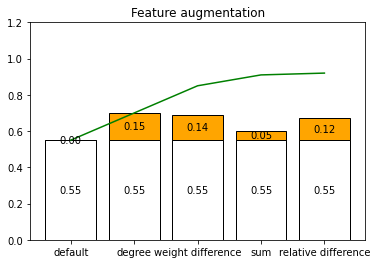
\includegraphics[scale=1.0]{figures/FeatureAugmentationLine}
    \caption{MNIST trained model. Average performance on 100 MNIST graphs}
    \label{Feature Augmentation Effect}
\end{figure}

With fine tuning og the models hyperparameters and architecture, and augmenting node features having the most effect on the performance, results were moving closer to reasonable. Now full training sets could be used. Unfortunately line graph transformation on a dense graph turned out to expode in size and take to much time to proccess. Therefore another architecture was considered.
 
\section{Edge prediction model}

Instead of turning edges to nodes model can give prediction in the node pair directly. With this approach there is less preprocessing needed, but the model now needs to have an extra layer for edge prediction as described in \hyperref[sec:architecture]{Aarchitecture section}.
After training both edge classification model and line graph model on the 55000 MNIST graphs following results were recorded: 88\% for edge classification and 92\% for line graph.

REDO !!! MNIST trained Model's performance on unseen MNIST graphs
\begin{figure}[H]
    \centering
    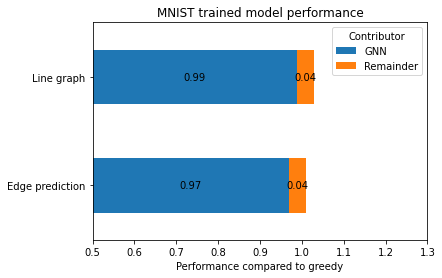
\includegraphics[scale=1.0]{figures/FinalPerformanceMNIST}
    \caption{MNIST performance comparison}
    \label{Model performance on MNIST}
\end{figure}

Edge classification showed a little bit worse results on average than the line graph. In theory it can be due to line graph containing more structural information in it compared to original. Regardless of the slightly worse result edge classification approach was still favourable due to time consumption of the line graph convertion. Naturally, the results are not ideal and further improvements are required. Additionaly due to size of MNIST graphs finding optimal solution using Blossom algorithm takes less time than using this \gls{gnn} model. The model however does catch up timewise when larger graphs are used. 

REDO !!! 
\begin{figure}[H]
    \centering
    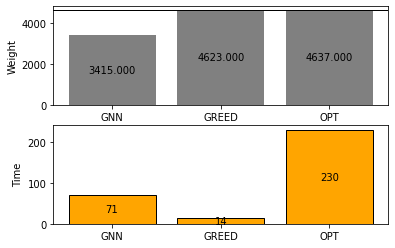
\includegraphics[scale=1.0]{figures/MNISTtrainSAGE10}
    \caption{MNIST trained model performance on sage10 graph}
    \label{model performance}
\end{figure}

As seen on the figure above \gls{gnn} manages to beat the optimal solver in term of time, but it is noticeably worse in terms of total weight. Poor performance can be because of the training dataset. One of the main interests was to see if the \gls{gnn} can be used on graphs larger than the ones it was trained on. It could be that model fails to learn what is needed for larger graphs. Another reason could be that MNIST graphs have similar structure without enough variety to cover other graph type. One ofcourse cannot include all the possible graphs in the training set, but the more data and variety model gets during training the better. Therefore another dataset was tried for training. A custom dataset consisting of randomly picked graphs from the SuiteSparse database. This custom dataset consists of 1000+ graphs with varying sizes and structures, between 100 and 10000 nodes.

Training the same model on the new dataset gave following results:
ADD FIGURE !!! RESULTS ON MNIST

REDO FIGURE !!!
\begin{figure}[H]
    \centering
    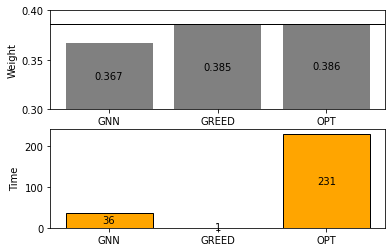
\includegraphics[scale=1.0]{figures/CUSTOMtrainSAGE10}
    \caption{CUSTOM trained model performance on sage10 graph}
    \label{model performance}
\end{figure}

With results still being unsatisfying, last improvement attempts were made.

Trying to add a reduction rule and 2 additional features: 1st largest weight, 2nd largest weight for each node.

ADD FIGURE !!! RESULTS FOR THE REDUCTION

Adjusting the threshold for the picking edges in to the solution and trying to remove edges below secondary threshold:
REDO FIGURE !!!
\begin{figure}[H]
    \centering
    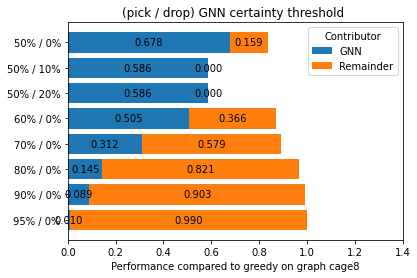
\includegraphics[scale=1.0]{figures/ThresholdDemo}
    \caption{Model performance on sage10 graph}
    \label{Model performance on sage10 graph}
\end{figure}

\section{Final results}

With time and ideas for further improvements staring to end, the final best model was tested on increasingly larger graphs. The final parameters of the model were:

\begin{enumerate}
\item Learning rate = 0.001
\item Network depth and width = 2 layers, 640 neurons each
\item Class weights = 0.1 and 0.9 for excluded and included in solution respectively
\item Weight decay = 0
\item Added pre computed node features
	\begin{itemize}
	\item Degree - how many neighbours a node has
	\item Weight relative to the sum of neighbours.
	\item Weight difference from the sum of the neighbours.
	\item Sums of the weights. 
	\end{itemize}
\end{enumerate}

ADD FIGURE !!! Final and best model trained using custom dataset on increasingly larger graphs:

\subsection{Weakness of greedy algorithm}

On average greedy seems to show realy good results, but in theory it is not hard to make a graph that abuses the greedy approach and results in poor performance. Example of a graph that \gls{gnn} model should be able to beat:

\begin{figure}[H]
    \centering
    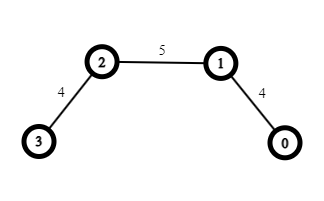
\includegraphics[scale=1.0]{figures/GoodCase}
    \caption{Good case for GNN}
    \label{Good case for GNN}
\end{figure}

In this very simple case the greedy algorithm will result in total weight = 5. Yet the \gls{gnn} does manage to get the optimal weight = 8. This ofcourse does not neccesarily prove anything, but shows that there might be use cases for the model. 

Additionaly, given that the runing times of greedy and \gls{gnn} combined are still lower than running time of finding the optimal solution, one may even run both and choose the better result.